The new method for homographiy resampling is based on the decomposition of an homography which can be seen as camera moves. The section below presents that decompostion.


%La nouvelle méthode de traitement des homographies repose sur la décomposition d'une homographie qui permet d'interpréter cette dernière en terme de mouvement de caméra. La partie ci-dessous présente cette décomposition.

\ssse{Modelisation of a camera mouvement}
%\ssse{Modélisation de mouvement de caméra}
\label{mouv_de_camera}

An \emph{a priori} special case of homographies $h$ that can be viewed as an ideal camera movement is studied there. It will be shown afterward the it is a general case.
%On étudie ici un cas a priori particulier d'homographie $h$ : les homographies que l'on peut interpréter comme un mouvement de caméra idéale. On montrera par la suite que c'est en fait un cas général.

Assume that the filmed scene is a plane. This assume that the filmed scene does not have any relief, or that the relief is negligible with respect to the distance between the plan and the camera, so that the relief is not seen. The figure \ref{shmdecomp} illustrates the modelisation of the ideal camera. Therefore the ideal camera can be seen as the projection of a plane on another plane by going throughout the focus $F$, without taking all the lens and electronic systems that are in real camera into account.

%Nous modéliserons la situation en supposant que la scène filmée est plane. Cela suppose que l'on filme une surface soit sans aucun relief, soit avec un relief négligeable devant la distance à la caméra, afin qu'il ne soit pas perceptible. La figure \ref{shmdecomp} illustre la modélisation utilisée pour la caméra idéale. La caméra idéale se modélise donc par la projection d'un plan sur un autre en passant par un foyer $F$, en négligeant les lentilles ou les dispositifs correcteurs présents dans les caméras réelles.

\begin{figure}[h!]

\centering
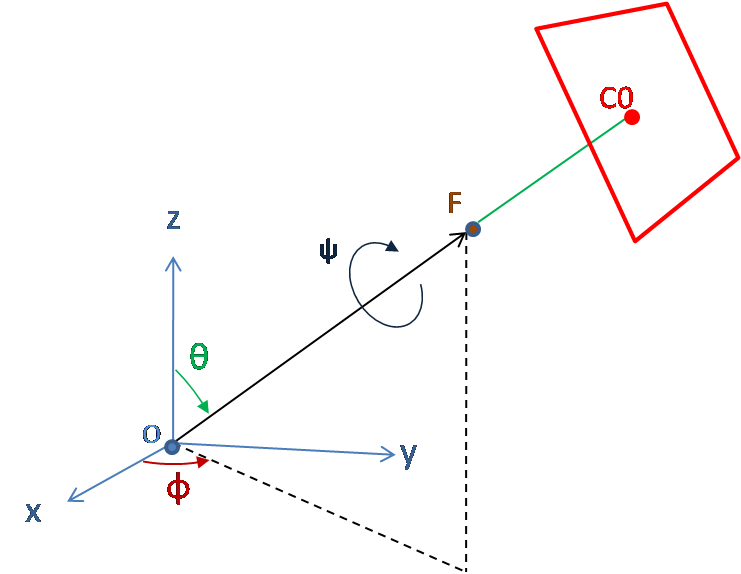
\includegraphics[width=10cm]{shema_decomp.png}
\caption{Illustration of a camera mouvement $(X_v =0)$ (In order to be clearer the translations have not been shown. $F$ is the focus of the camera, the red plane is the image plane of the camera.  One point of the image plane is obtained by the projection of a point of the plane $(x,y)$ through the point $F$. (cf. part \ref{mouv_de_camera})}
\label{shmdecomp}
\end{figure}

Let's consider the vector space $\mathbb{R}^{3}$  of $O$ the origin $(0,0,0)$  and $(\xbf_0,\ybf_0,\zbf_0)$ the standard basis.
%On se place dans l'espace vectoriel $\mathbb{R}^{3}$ on note $O$ l'origine $(0,0,0)$ et $(\xbf_0,\ybf_0,\zbf_0)$ la base canonique.
\begin{itemize}
\item Let $F$ and $C_0$ be two differents points in $\mathbb{R}^{3}$.
\item Let $\mathcal{P}$ be the affine plane through $C_0$ and of normal vector $\overrightarrow{FC_0}$.
\item Let $\wbf$ be the vector $\frac{\overrightarrow{FC_0}}{|| \overrightarrow{FC_0}||}$
\item Let $\delta$ be the distance $|| \overrightarrow{FC_0}||$
\end{itemize}
\begin{Def}
The projective mapping $H$, is the mapping which receives a point $X$ in $\mathbb{R}^{3}$ and return point of intersection of the straight line $(XF)$ and the plane $\mathcal{P}$. $H$ depends on $(F,\wbf,\delta)$.
%L'application projective $H$, est l'application qui à un point $X$ de $\mathbb{R}^{3}$ associe le point d'intersection entre la droite $(XF)$ et le plan $\mathcal{P}$. $H$ dépend du triplet $(F,\wbf,\delta)$.
\end{Def}
\begin{remarques}
\begin{itemize}
\item $F$ is the position of the focus of the camera and the plane $\mathcal{P}$ is the plane of the camera on which the image is projected. The optical axis of the camera is the straight line $(FC_0)$ of direction vector $\wbf$, $\delta$ is the the distance between the focus and the screen.
\item From A a point in $\mathbb{R}^3$, the mapping $H$ return the point of $\mathcal{P}$ corresponding to it's image troughout the camera.
\end{itemize}
\end{remarques}
Let $\mathcal{P}'$ be the affine plane of $\mathbb{R}^{3}$ containing $F$ and parallel to the plane $\mathcal{P}$.
\begin{lem}
$H$ is defined on $\mathbb{R}^3 \setminus \mathcal{P}'$ and,
\begin{equation}
H(X) = C_0 +  \delta \frac{\overrightarrow{XF}-(\overrightarrow{XF}\cdot \wbf )\wbf}{\wbf \cdot \overrightarrow{XF}.} 
\label{formul_lem_app_proj}
\end{equation}
\label{lem_app_proj}
\end{lem}
\begin{proof}
If $X\in \mathbb{R}^3 \setminus \{F\}$ the straight ligne $(XF)$ and have an intersection point with $\mathcal{P}$ if and only if it is not parallel to  $\mathcal{P}$ so if and only if $X\in \mathbb{R}^3 \setminus \mathcal{P}'$. In that case, there exists $t_X\in \mathcal{R}$ such that
\begin{equation*}
H(X)=X+t_{X}\overrightarrow{XF}.
\end{equation*}
As $H(X)\in P_{2}$ then
\begin{equation*}
\overrightarrow{FH(X)}\cdot \wbf =\delta.
\end{equation*}
By using the formula of $H(X)$ one can obtain
\begin{equation*}
t_{X}=1+\frac{\delta}{\wbf \cdot \overrightarrow{XF}},
\end{equation*}
 Then it can be deduced that
\begin{equation*}
H(X) = C_0 +  \delta \frac{\overrightarrow{XF}-(\overrightarrow{XF}\cdot \wbf )\wbf}{\wbf \cdot \overrightarrow{XF}}.
\end{equation*}
\end{proof}
\begin{remarque}
The plane $\mathcal{P}'$ is the blindspot of the camera ; in the case of a real camera, that blindspot should be all what is behind the camera.
\end{remarque}
Let $P$ be the plan $(O,\xbf_0,\ybf_0)$.
\begin{Def} Let's call target point the intersection point of the straight line $(FC_0)$ and the plane $P$ if it exists. The target point exists if and only if $(FC_0)$ is not parallel to $\mathcal{P}$. When it exists it is called $X_v$ and then
\begin{equation*}
X_v=F-\wbf \delta'~~~~~~\delta'=\frac{\overrightarrow{OF}\cdot \zbf_0}{\wbf \cdot \zbf_0}
\label{formule_point_vise}
\end{equation*}
\label{point_vise}
\end{Def}
\begin{remarque}
The target point is the point $P$ targetted by the camera, the camera movements are such that the camera is always targetting that point. It is possible that a camera does not have a target point, in that case the point is at infinity, the camera targets the horizon.
\end{remarque}
Assume for what's next that the target point exists.
\begin{Def}
The projective planar mapping $H^*$ related to $H$ is the restriction of $H$ to $P\setminus (\mathcal{P}'\cap P)$. 
If $\wbf \perp P $, then $H^*$ is defined on $P$. Otherwise $H^*$ is defined on $P\setminus D$ where $D$ is the straight line
\begin{equation*}
D=\left\{ X\in P | \overrightarrow{XF}\cdot \wbf = 0\right\}.
\end{equation*}
\end{Def}
\begin{remarques}
\begin{itemize}
\item Let's say that the filmed scene is close enough to a plane so that any relief is negligible and can be interpreted as the plane $P$. Then, from a point $X\in P$ of the filmed scene, the mapping $H^*$ returns the point in $P_2$ which is its image throughout the camera.
\item The straight line $D'=\{ X \in \mathcal{P} | \overrightarrow{XF} \cdot \zbf_0 =0 \}$ is called the horizon of $H^*$.
\end{itemize}

\end{remarques}
Let's give to the affine plane $\mathcal{P}$ a direct normalized basis $(C,\ubf,\vbf)$. 
\begin{Def}
 The homography related with $H^*$ in the basis $(C,\ubf,\vbf)$ is the mapping
\begin{equation}
h : (x,y)  \mapsto \left( \overrightarrow{CH^*(X)}\cdot \ubf , \overrightarrow{CH^*(X)}\cdot \vbf \right)
\label{formule_homographie_H}
\end{equation}


whith $X=x~\xbf_0 + y~\ybf_0 $.
\label{def_homographie_H}
\end{Def}
Let $D,D'$ be the sraight lines in $\mathbb{R}^2$ obtained when $P$ and $\mathcal{P}$ have the basis $(O,\xbf,\ybf)$ and $(C,\ubf,\vbf)$ then $h:\mathbb{R}^2  \setminus D \mapsto \mathbb{R}^2  \setminus D'$ is a bijective mapping.
\begin{remarque}
From a point $X\in P$ of coordinates $(x,y)$  the mapping $h$ return the coordinates of the point $H^*(X)$ of the numeric image coming from the camera. 
\end{remarque}
The orientation of the basis $(\ubf,\vbf,\wbf)$ with respect to the basis $(\xbf_0,\ybf_0,\zbf_0)$ can be defined by the three Euler anglespeut être définie grâce aux trois angles d'Euler $(\phi , \theta ,\psi )$ (figure \ref{img_angles})
\begin{itemize}
\item $\phi$ est is the first rotation around the axis $(X_v ,\zbf_0)$
\item $\theta$ is the second rotation around to the axis $(X_v , \zbf_0 )$
\item $\psi$ est is the third rotation around the axis $(X_v , \wbf )$
\end{itemize}
On note $\cbf= \left (\overrightarrow{C_0 C}\cdot \ubf , \overrightarrow{C_0 C}\cdot \vbf \right)$ et $\xbf_v=\left( \overrightarrow{O X_v}\cdot \ubf , \overrightarrow{O X_v}\cdot \vbf \right )$.\\
\begin{prop}
The homography $h$ can be factorized as follows
 
\begin{equation}
h = \tau_{\cbf}   \circ R_{\psi} \circ z_{\frac{\delta}{\delta'}} \circ h_{\theta,\delta'} \circ R_{\phi} \circ \tau_{\xbf_v}
\label{formul_decomp}
\end{equation}
 $R_{\alpha}$ is the rotation is the rotation of angle $\alpha$,$z_\lambda$ is the zoom of factor $\lambda$, $\tau_\ybf$ and the translation along the vector $-\ybf$ and $h_{\theta,\delta'}$ is the undirectional homography (cf. definition \ref{homo_uni_direc})
\begin{equation}
h_{\theta,\delta'}(x,y)=\left(\frac{-cos(\theta)x}{1-\frac{sin(\theta)}{\delta'}x} ,\frac{-y}{1-\frac{sin(\theta)}{\delta'}x}\right)
\label{mise_perspective}
\end{equation}
\label{prop_decomp}
\end{prop}
\begin{Def}
A unidirectional homography is a mapping $h:\mathbb{R}^{2} \ra \mathbb{R}^{2}$ defined by
\begin{equation*}
h(x,y)=\left ( \frac{ax+p}{rx+t} , \frac{cy+p}{rx+t} \right)
\end{equation*}
with $a,p,c,q,r,t$ some reals numbers.
\label{homo_uni_direc}
\end{Def}
\begin{figure}[h!]
\centering
\subfigure[rotation of angle $\phi$]{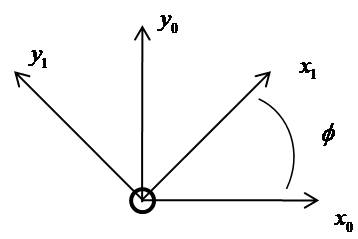
\includegraphics[width=5cm]{graphe1.jpg}}
\subfigure[rotation of angle $\theta$]{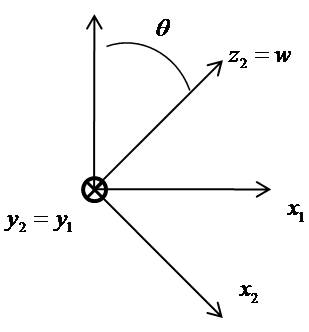
\includegraphics[width=5cm]{graphe2.jpg}}
\caption{(cf part \ref{figure_de_rotations_18})}
\label{img_angles}
\end{figure}

\begin{figure}[h!]
\centering
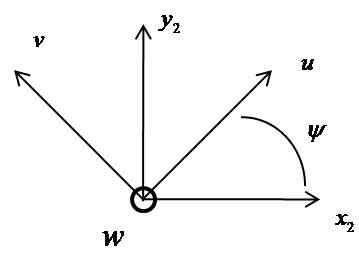
\includegraphics[width=5cm]{graphe3.jpg}
\caption{self rotation (cf part \ref{figure_de_rotations_18})}
\label{decompgeo_rotationPropre}
\end{figure}





\begin{proof}
Using formula (\ref{formule_homographie_H}), definition (\ref{def_homographie_H}) and the formula (\ref{formul_lem_app_proj}) of the lemma (\ref{lem_app_proj}), we have
\begin{equation*}
h((x,y))=\left( \delta \frac{\overrightarrow{XF}\cdot \ubf}{\overrightarrow{XF} \cdot \wbf} +\overrightarrow{CC_0 } \cdot \ubf, \delta \frac{\overrightarrow{XF}\cdot \vbf}{\overrightarrow{XF} \cdot  \wbf}+\overrightarrow{CC_0 }\cdot \vbf \right)
\end{equation*}
where $X=x \xbf_0 + y \ybf_0 $.\\

By introducing the target point $X_v$ (definition \ref{point_vise} formula \ref{formule_point_vise}) and the translation $\tau_c$ we have
\begin{equation}
(\tau_\cbf^{-1} \circ h)((x,y)) = \left ( -\delta \frac{\overrightarrow{X_vX}\cdot \ubf}{\delta' -\overrightarrow{X_vX} \cdot \wbf},-\delta \frac{\overrightarrow{X_vX}\cdot \vbf}{\delta' -\overrightarrow{X_vX} \cdot \wbf} \right)
\label{decomp_formul_intermediaire_1}
\end{equation}


Intermediate basis $(\xbf_1 ,\ybf_1 ,\zbf_1)$  $(\xbf_2 ,\ybf_2 ,\zbf_2)$ can be defined, in order to decompose the three rotations $\phi,\theta,\psi$ (figures \ref{img_angles} and \ref{decompgeo_rotationPropre} ).

Then we have the relations
\begin{equation*}
\ubf=\cos(\psi)\xbf_{2}+\sin(\psi)\ybf_{2} , \vbf=-\sin(\psi)\xbf_{2}+\cos(\psi)\ybf_{2} \text{ et } \wbf=\zbf_2.
\end{equation*}

Denoting $R_{s}$ the rotation of angle $s$, we obtained, by using the formula (\ref{decomp_formul_intermediaire_1}) 
\begin{equation*}
(\tau_{\cbf}^{-1} \circ h)((x,y)) = R_{\psi}\left(\frac{\delta \overrightarrow{X_v X}\cdot \xbf_{2} }{\delta'-\zbf_2 \cdot \overrightarrow{X_v X}},\frac{\delta \overrightarrow{X_v X}\cdot \ybf_{2}}{\delta'-\zbf_2 \cdot \overrightarrow{X_v X}}  \right).
\end{equation*}
Let $i$ be the mapping such that $i(x,y)=x \xbf_0 + y \ybf_0$. Since $i(\xbf_v)=\overrightarrow{O X_v}$ we have
\begin{equation*}
(R_{\psi}^{-1} \circ \tau_{\cbf}^{-1}  \circ h)((x,y))=\delta \left(\frac{-i(\tau_{\xbf_v} ((x,y)))\cdot \xbf_{2} }{\delta'-\zbf_2 \cdot i(\tau_{\xbf_v} ((x,y)))},\frac{-i(\tau_{\xbf_v} ((x,y)))\cdot \ybf_{2}}{\delta'-\zbf_2 \cdot i(\tau_{\xbf_v} ((x,y)))}  \right) 
\end{equation*}

Since $\zbf_{2}=cos(\theta)\zbf_{1}+sin(\theta)\xbf_{1}$, $\xbf_{2}=cos(\theta)\xbf_{1}-sin(\theta)\zbf_{1}$ (figure \ref{img_angles}) and $\zbf_{1}\perp P_{1}$, we have

\begin{equation*}
(R_{\psi}^{-1} \circ \tau_{\cbf}^{-1}  \circ h)((x,y))=\frac{\delta}{\delta'}\left(\frac{-\cos(\theta)i(\tau_{\xbf_v} ((x,y)))\cdot \xbf_{1} }{1-\frac{sin(\theta)}{\delta'}\xbf_{1}\cdot i(\tau_{\xbf_v}((x,y)))}, \frac{-i(\tau_{\xbf_v} ((x,y)))\cdot \ybf_{1}}{1-\frac{sin(\theta)}{\delta'}\xbf_{1}\cdot i(\tau_{\xbf_v}((x,y)))}  \right) 
\end{equation*}

Let $h_{\theta,\delta'}$ be defined by

\begin{equation*}
h_{\theta,\delta'}(x',y')=\left(\frac{-\cos(\theta)x'}{1-\frac{\sin(\theta)}{\delta'}x'} ,\frac{-y'}{1-\frac{\sin(\theta)}{\delta'}x'}\right)
\end{equation*}

Then

\begin{equation*}
(R_{\psi}^{-1} \circ \tau_{\cbf}^{-1} \circ h)((x,y))= \frac{\delta}{\delta'}h_{\theta,\delta'}\left ( i(\tau_{\xbf_v}((x,y))) \cdot \xbf_{1}, i(\tau_{\xbf_v}((x,y))) \cdot \ybf_{1}\right)
\end{equation*}
\label{figure_de_rotations_18}
Since $\xbf_{1}=\cos(\phi)\xbf_{0}+\sin(\phi)\ybf_{0}$ et $\ybf_{1}=-\sin(\phi)\xbf_{0}+\cos(\phi)\ybf_{0}$ (figure \ref{img_angles}), we have

\begin{eqnarray*}
(R_{\psi}^{-1} \circ \tau_{\cbf}^{-1} \circ h)((x,y)) &=& \frac{\delta}{\delta'}h_{\theta,\delta'}\left ( R_{\phi}(i(\tau_{\xbf_v}((x,y))) \cdot \xbf_{0}, i(\tau_{\xbf_v}((x,y))) \cdot \ybf_{0})\right)\\
                                               &=&\frac{\delta}{\delta'} (h_{\theta,\delta'}\circ R_{\phi} \circ \tau_{\xbf_v})((x,y))
\end{eqnarray*}

Denoting zooms $z_{\lambda}:X\rightarrow \lambda X$, the claim is verified since

\begin{equation*}
h = \tau_{\cbf} \circ R_{\psi} \circ z_{\frac{\delta}{\delta'}} \circ h_{\theta,\delta'} \circ R_{\phi} \circ \tau_{\xbf_v}
\end{equation*}

\end{proof}


\begin{remarques}
\begin{itemize}
\item Resampling an image by the homography $h$ simulate a change of the point of view on the input image. This has parameters $(\phi,\theta,\psi,\delta,\delta',\xbf_v,\cbf_v)$, which are not independent.
\item The case in which the camera is targeting the horizon has not been discussed, translations $\tau_\cbf$ allow to avoid this.
\end{itemize}
\end{remarques}



\begin{remarque}
The previous method does not modeled every affine transform. Indeed the function $h$ defined by 
\begin{equation*}
h = \tau_{\cbf}   \circ R_{\psi} \circ z_{\frac{\delta}{\delta'}} \circ h_{\theta,\delta'} \circ R_{\phi} \circ \tau_{\xbf_v}
\end{equation*}
is affine if and only if $\theta=0$. In this case we have
\begin{equation*}
h= \tau_{\cbf} \circ z_{-\frac{\delta}{\delta'}} \circ R_{\phi+\psi} \circ \tau_{\xbf_{v}}
=\tau' \circ z_{-\frac{\delta}{\delta'}} \circ  R_{\phi+\psi}
\end{equation*}
However the affinity can be seen as a limit case. Let $k$ be the ratio $\frac{\delta}{\delta'}$. If $\delta'$ and $\delta$ tense to $+\infty$, the function $h_{\theta,\delta'}$, the function $h_{\theta,\delta'}$ tense to $h_{\theta,\infty}$ defined by
\begin{equation*}
h_{\theta,\infty}=(x,y)=(-\cos(\theta)x,-y)
\end{equation*}
Physically, it is equivalent to moving away from the plane while increasing the focal distance in order to keep the size of the output image constant.

If $h_\infty = z_{-\frac{\delta}{\delta'}} \circ \tau_{\xbf} \circ R_{\phi} \circ h_{\theta,\infty} \circ R_{\psi} \circ \tau_{\xbf_{v}}$, the linear part $h_{\infty}$ can be represented by a matrix $2\times2$

\begin{equation*}
R_{\psi} \cdot 
\begin{pmatrix}
-k\cos(\theta)&0\\
0&-k
\end{pmatrix}
\cdot R_{\phi}
\end{equation*}

If $M$ is an invertible matrix $2\times 2$, then we have the following lemma using the singular value decomposition \cite{morel2009asift}.
\begin{lem}
There exists two rotation matrix $R_1$ and $R_2$ and a diagonal matrix $D$ such that $M = R_1 \cdot D \cdot R_2$.
\label{decomp_valeur_sing}
\end{lem}

Using the lemma (\ref{decomp_valeur_sing}) it can be deduced that for all bijective affinity $A$, there exists a camera movement $h$ such that $h_\infty = A$. Moreover it can be assumed that $h$ has no output translation.
\end{remarque}






\subsubsection{Application of the decomposition to homographies}
The previous results show that all homographies can be decomposed using the following Theorem

%Le résultat précédent montre que certaine homographie peuvent se décomposer de la
\begin{thm}
Let $h$ be an homography, if $h$ is not an affine map then there exists parameters $(\phi,\theta,\psi,\delta,\delta',(x_1,y_1),(x_2,y_2))$ such that
\begin{equation*}
h = \tau_{(x_2,y_2)} \circ R_{\psi} \circ z_{\frac{\delta}{\delta'}} \circ h_{\theta,\delta'} \circ R_{\phi} \circ \tau_{(-x_1,-y_1)}
\end{equation*}
This decomposition is not unique. More precisely for all $\lambda \in ]0,1[$,

  \begin{equation*}
h = \tau_{(x_2,y_2)} \circ z_{\frac{\delta}{\delta'}}  \circ R_{\psi} \circ h_{\theta,\delta'} \circ R_{\phi} \circ \tau_{(-x_1,-y_1)}
  \end{equation*}
  where 
 \begin{equation*}
x_2=\frac{ar+sb+\hat r \lambda}{r^2 +s^2}, y_2=\frac{cr+sd+\hat s \lambda}{r^2 +s^2}, (x_1 , y_1) = h^{-1}(x_{2},y_{2})
  \end{equation*}
 \begin{equation*}
 \cos( \phi )= - \frac{r}{\sqrt{r^2 + s^2}}, \sin( \phi )= - \frac{s}{\sqrt{r^2 + s^2}},\cos( \psi ) =- \frac{\hat r}{\sqrt{\hat r^2 + \hat s^2}}, \sin( \psi ) = \frac{\hat s}{\sqrt{\hat r^2 + \hat s^2}}
 \end{equation*}
 \begin{equation*}
 \frac{\delta}{\delta'}=|\lambda|\sqrt{\frac{\hat r^2 + \hat s^2}{r^2 + s^2}}^{3}, \cos(\theta)=\lambda, \sin(\theta)=\sqrt{1-\lambda^2}, \delta'=  \frac{\sqrt{(r^2 + s^2)(1-\lambda^2)}}{|\lambda| (\hat r^2+\hat s^2)}
 \end{equation*}
\label{thepropdecomp}
\end{thm}

\begin{corollaire} If $h$ an homography and $h$ is not affine, then there exists a translation $\tau$, two rotations $R_\phi ,R_\psi$ and a unidirectional homography $\tilde{h}$ such that
\begin{equation}
h=\tau \circ R_\psi \circ \tilde{h} \circ R_\phi
\label{formule_decomposition_effective}
\end{equation}
and this decomposition is not unique.
\end{corollaire}

		This formula is used in the algorithm \ref{pseudoCodeDecompo}.
		
		\begin{proof}
	 Using theorem (\ref{thepropdecomp}),there exists $(\phi,\theta,\psi,\delta,\delta',\xbf_v,\cbf)$ such that 
	 \begin{equation*}
	 h = \tau_{\cbf} \circ R_{\psi} \circ z_{\frac{\delta}{\delta'}} \circ h_{\theta,\delta'} \circ R_{\phi} \circ \tau_{\xbf_v}
	 \end{equation*}
	 $R_\psi$ and $z_{\frac{\delta}{\delta'}}$ commute. Let $\tau'$ be the theorem such that $\tau' \circ R_\phi =  R_\phi \circ \tau_{\xbf_v}$.\\
	 Then with $\tilde{h} = z_{\frac{\delta}{\delta'}} \circ 
	 h_{\theta,\delta'} \circ \tau'$ it can be easily verified that $\tilde{h}$ is indeed a unidirectional homography.
	 \end{proof}
	\label{ref_schema_decomp_cool}
	\begin{figure}
		\centering
		\subfigure[Input image]{
		\centering
		{
\includegraphics[scale=0.24]{vue_fps_identity.png}}
		{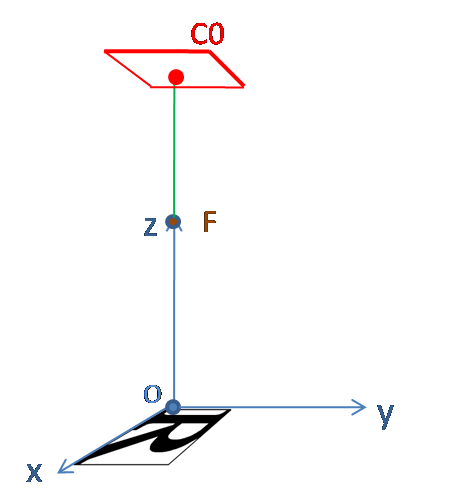
\includegraphics[scale=0.35]{vue_tps_identity.png}}}
		\subfigure[After a first rotation (of angle $\phi$)]{
		\centering
		{
\includegraphics[scale=0.24]{vue_fps_rotation_phi.png}}
		{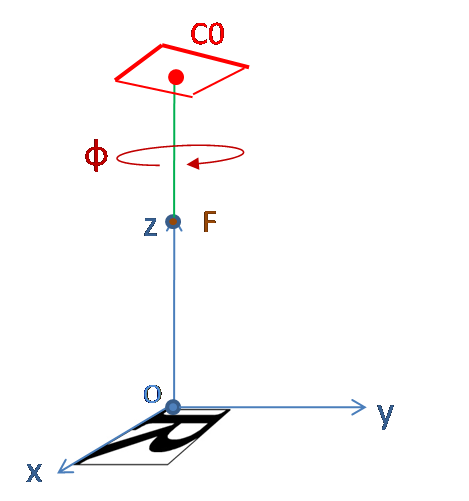
\includegraphics[scale=0.35]{vue_tps_rotation_phi.png}}}
		\subfigure[After the unidirectional homography]{
		\centering
		{
\includegraphics[scale=0.24]{vue_fps_hom_part.png}}
		{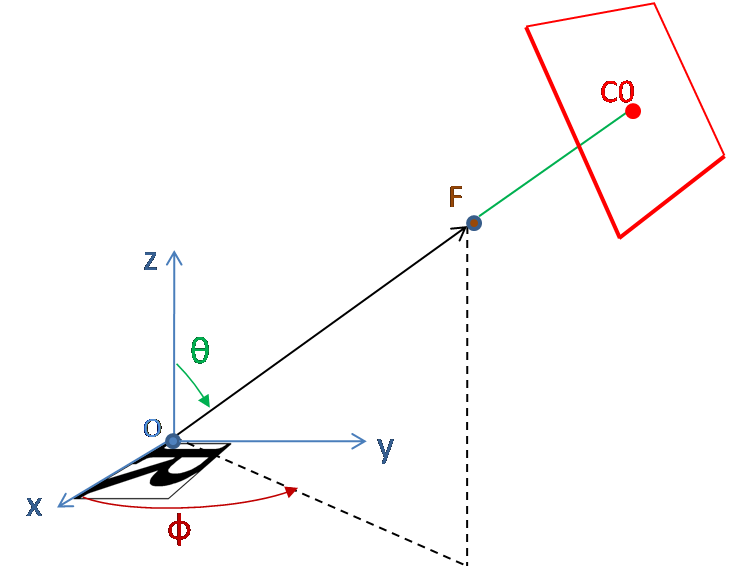
\includegraphics[scale=0.35]{vue_tps_hom_part.png}}}
		\subfigure[Output image (after the rotation of angle  $\psi$)]{
		\centering
		{
\includegraphics[scale=0.24]{vue_fps_rotation_psi.png}}
		{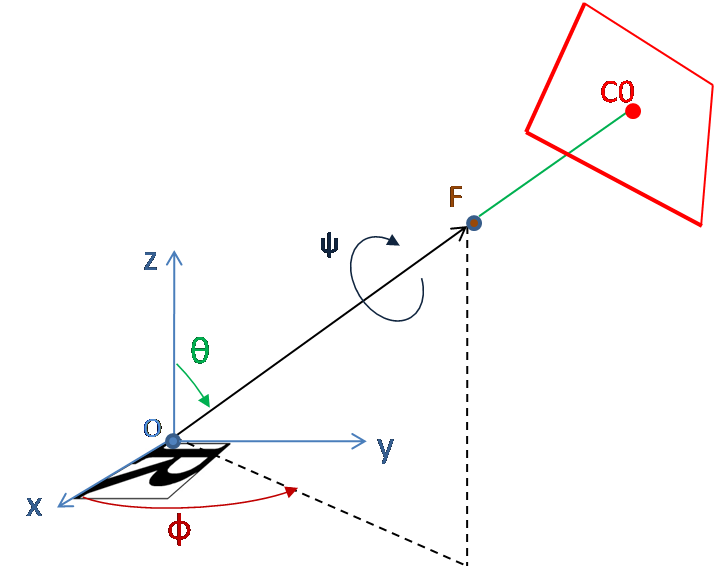
\includegraphics[scale=0.35]{vue_tps_rotation_psi.png}}}
		\caption{Steps to process an homography, represented as camera moves, on the left the view from the camera, on the left a motionless point of view. The translations are not represented to simplify the situation. On motionless views, $F$ is the focus of the camera, the red plane is the image plane of the camera. (cf. \ref{ref_schema_decomp_cool})}
		\label{schema_decomp_cool}
		\label{SchemaEtapesDecompoGeometrique}
	\end{figure}
	\clearpage
